% Options for packages loaded elsewhere
\PassOptionsToPackage{unicode}{hyperref}
\PassOptionsToPackage{hyphens}{url}
%
\documentclass[
]{article}
\usepackage{amsmath,amssymb}
\usepackage{iftex}
\ifPDFTeX
  \usepackage[T1]{fontenc}
  \usepackage[utf8]{inputenc}
  \usepackage{textcomp} % provide euro and other symbols
\else % if luatex or xetex
  \usepackage{unicode-math} % this also loads fontspec
  \defaultfontfeatures{Scale=MatchLowercase}
  \defaultfontfeatures[\rmfamily]{Ligatures=TeX,Scale=1}
\fi
\usepackage{lmodern}
\ifPDFTeX\else
  % xetex/luatex font selection
\fi
% Use upquote if available, for straight quotes in verbatim environments
\IfFileExists{upquote.sty}{\usepackage{upquote}}{}
\IfFileExists{microtype.sty}{% use microtype if available
  \usepackage[]{microtype}
  \UseMicrotypeSet[protrusion]{basicmath} % disable protrusion for tt fonts
}{}
\makeatletter
\@ifundefined{KOMAClassName}{% if non-KOMA class
  \IfFileExists{parskip.sty}{%
    \usepackage{parskip}
  }{% else
    \setlength{\parindent}{0pt}
    \setlength{\parskip}{6pt plus 2pt minus 1pt}}
}{% if KOMA class
  \KOMAoptions{parskip=half}}
\makeatother
\usepackage{xcolor}
\usepackage[margin=1in]{geometry}
\usepackage{longtable,booktabs,array}
\usepackage{calc} % for calculating minipage widths
% Correct order of tables after \paragraph or \subparagraph
\usepackage{etoolbox}
\makeatletter
\patchcmd\longtable{\par}{\if@noskipsec\mbox{}\fi\par}{}{}
\makeatother
% Allow footnotes in longtable head/foot
\IfFileExists{footnotehyper.sty}{\usepackage{footnotehyper}}{\usepackage{footnote}}
\makesavenoteenv{longtable}
\usepackage{graphicx}
\makeatletter
\def\maxwidth{\ifdim\Gin@nat@width>\linewidth\linewidth\else\Gin@nat@width\fi}
\def\maxheight{\ifdim\Gin@nat@height>\textheight\textheight\else\Gin@nat@height\fi}
\makeatother
% Scale images if necessary, so that they will not overflow the page
% margins by default, and it is still possible to overwrite the defaults
% using explicit options in \includegraphics[width, height, ...]{}
\setkeys{Gin}{width=\maxwidth,height=\maxheight,keepaspectratio}
% Set default figure placement to htbp
\makeatletter
\def\fps@figure{htbp}
\makeatother
\setlength{\emergencystretch}{3em} % prevent overfull lines
\providecommand{\tightlist}{%
  \setlength{\itemsep}{0pt}\setlength{\parskip}{0pt}}
\setcounter{secnumdepth}{-\maxdimen} % remove section numbering
\usepackage{multicol}
\usepackage{longtable}
\setlength{\columnsep}{1cm}
\usepackage{booktabs}
\usepackage{array}
\usepackage{float}
\usepackage{longtable}
\usepackage{multirow}
\usepackage{wrapfig}
\usepackage{colortbl}
\usepackage{pdflscape}
\usepackage{tabu}
\usepackage{threeparttable}
\usepackage{threeparttablex}
\usepackage[normalem]{ulem}
\usepackage{makecell}
\usepackage{xcolor}
\ifLuaTeX
  \usepackage{selnolig}  % disable illegal ligatures
\fi
\usepackage{bookmark}
\IfFileExists{xurl.sty}{\usepackage{xurl}}{} % add URL line breaks if available
\urlstyle{same}
\hypersetup{
  pdftitle={Análisis de Variables que Influyen en la Inversión, Innovación e Implementación de la Inteligencia Artificial},
  hidelinks,
  pdfcreator={LaTeX via pandoc}}

\title{Análisis de Variables que Influyen en la Inversión, Innovación e
Implementación de la Inteligencia Artificial}
\author{Adrada Isabel, De la Peña Juan, Terán Federico, Troncoso
Samuel\\
Pontificia Universidad Javeriana Cali}
\date{}

\begin{document}
\maketitle

\begin{multicols}{2}

\section{Resumen}
Este estudio analiza las variables clave que influyen en la inversión, innovación e implementación de la inteligencia artificial (IA) a nivel global, utilizando el AI Global Index como referencia. Mediante un análisis estadístico descriptivo y correlacional, se identificaron los índices Commerce (inversión), Research (innovación) y Talent (implementación) como factores críticos, destacando su relación lineal significativa con el Total Score. Además, se exploró el impacto de la variable Región en la distribución geográfica del desarrollo de IA.

\section{Key words}
Inteligencia artificial, inversión, innovación, implementación, análisis estadístico.

\section{Introducción}
Las compañıas involucradas en el desarrollo tecnológico con inteligencia artificial (IA) necesitan identificar las regiones con mayor potencial de adopción e implementación de estas herramientas. Este análisis es crucial para la toma de decisiones estratégicas, la definición de mercados objetivo y la planificación de estrategias de expansión geográfica, razón por lo cuál, debido a la incertidumbre respecto a los factores con mayor impacto en el potencial éxito de los planes de expansión operativa en diferentes partes del mundo, se plantea el interrogante ¿Qué variables tienen mayor influencia en los niveles de inversión, innovación e implementación de la inteligencia artificial según lo reflejado en el AI Global Index [1] (índice que compara diferentes países en estos niveles), y cómo varía esta influencia según la región geográfica?.

El objetivo general de este estudio radica en identificar las variables con un mayor grado de influencia en el nivel de inversión, innovación e implementación de la inteligencia artificial, reflejado en el AI global index de diferentes regiones del mundo, por lo cuál, en primera instancia se identificaron los índices para cada factor mencionado con un mayor coeficiente de correlación lineal de Pearson de acuerdo a la metodología e interpretación plaenteada por Navidi [2], permitiendo el plateamiento de los objetivos específicos con el fin de determinar la influencia de los factores relacionados con la inversión mediante el índice Commerce, la innovación mediante el índice Research, la implementación mediante el índice Talent y la ubicación geográfica del país mediante la categorización por Región.

A partir de los anteriores planteamientos se formula como hipótesis: la influencia del nivel de inversión (índice Commerce), innovación (índice Research) e implementación (índice Talent) de inteligencia artificial en el desempeño de los países según el AI Global Index (Total Score) presenta diferencias altamente significativas según la región geográfica.




\section{Métodos}
Para la definición de las variables a estudiar a partir de la base de datos AI Global Index trabajada en el presente estudio, se relalizó una exploración preliminar de los datos en la Tabla 1, donde se nombran las variables, se clasifican como cualitativas o cuantitativas, se categorizan como continuas o discretas, o nominal u ordinal según el caso y se realiza una descripción de las mismas.

\end{multicols}

\renewcommand{\arraystretch}{1.5}
\begin{footnotesize}
\begin{longtable}[t]{lllp{8cm}}
\caption{\label{tab:tabla1}Variables y su clasificación}\\
\toprule
Variable & Clasificación & Categorización & Descripción\\
\midrule
Country & Cualitativa & Nominal & Nombre del país donde se evalúa el AI Global Index.\\
Talent & Cuantitativa & Continua & Indicador de disponibilidad de profesionales calificados para la provisión de soluciones de inteligencia artificial.\\
Infraestructure & Cuantitativa & Continua & Indicador de fiabilidad y la escala de la infraestructura de acceso, desde la electricidad e Internet, hasta las capacidades de superintarmética.\\
Operating Enviroment & Cuantitativa & Continua & Indicador del contexto regulatorio y la opinión pública en torno a la inteligencia artificial.\\
Research & Cuantitativa & Continua & Indicador del alcance de la investigación especializada y los investigadores; investigando la cantidad de publicaciones y citas en revistas académicas creíbles.\\
\addlinespace
Development & Cuantitativa & Continua & Indicador de desarrollo de plataformas y algoritmos fundamentales en los que se basan los proyectos innovadores de inteligencia artificial.\\
Government Strategy & Cuantitativa & Continua & Indicador de la profundidad del compromiso del gobierno nacional con la inteligencia artificial; investigando los compromisos de gasto y las estrategias nacionales.\\
Commerce & Cuantitativa & Continua & Indicador del nivel de actividad de puesta en marcha, inversión e iniciativas comerciales basadas en la inteligencia artificial.\\
Total Score & Cuantitativa & Continua & Indicador AI Global Index que compara a las naciones en su nivel de inversión, innovación e implementación de la inteligencia artificial.\\
Region & Cualitativa & Nominal & Agrupacion de países según su localización geográfica en regiones.\\
\addlinespace
Cluster & Cualitativa & Nominal & Agrupación de países según su historia de incursión en el desarrollo de tecnología relacionada con la Inteligencia Artificial.\\
Income Group & Cualitativa & Ordinal & Nivel de ingresos presentado en el país.\\
Political Regime & Cualitativa & Nominal & Tipo de régimen político presentado en el país.\\
\bottomrule
\end{longtable}

\end{footnotesize}\renewcommand{\arraystretch}{1}

\begin{multicols}{2}


Posteriormente, con el propósito de indentificar las posibles variables con un mayor grado de influencia en el nivel de inversión, innovación e implementación de la inteligencia artificial, se elaboró la Figura 1, la cuál presenta una comparación de las distribuciones de las variables y sus respectivos coeficientes de correlación lineal de Pearson con el fin de reconocer los índices que presentan un mayor valor respecto al AI Global Index (Total Score), los cuáles fueron Commerce para el nivel de inversión, Research para la innovación y Talent para la implemetación. 




\begin{center}
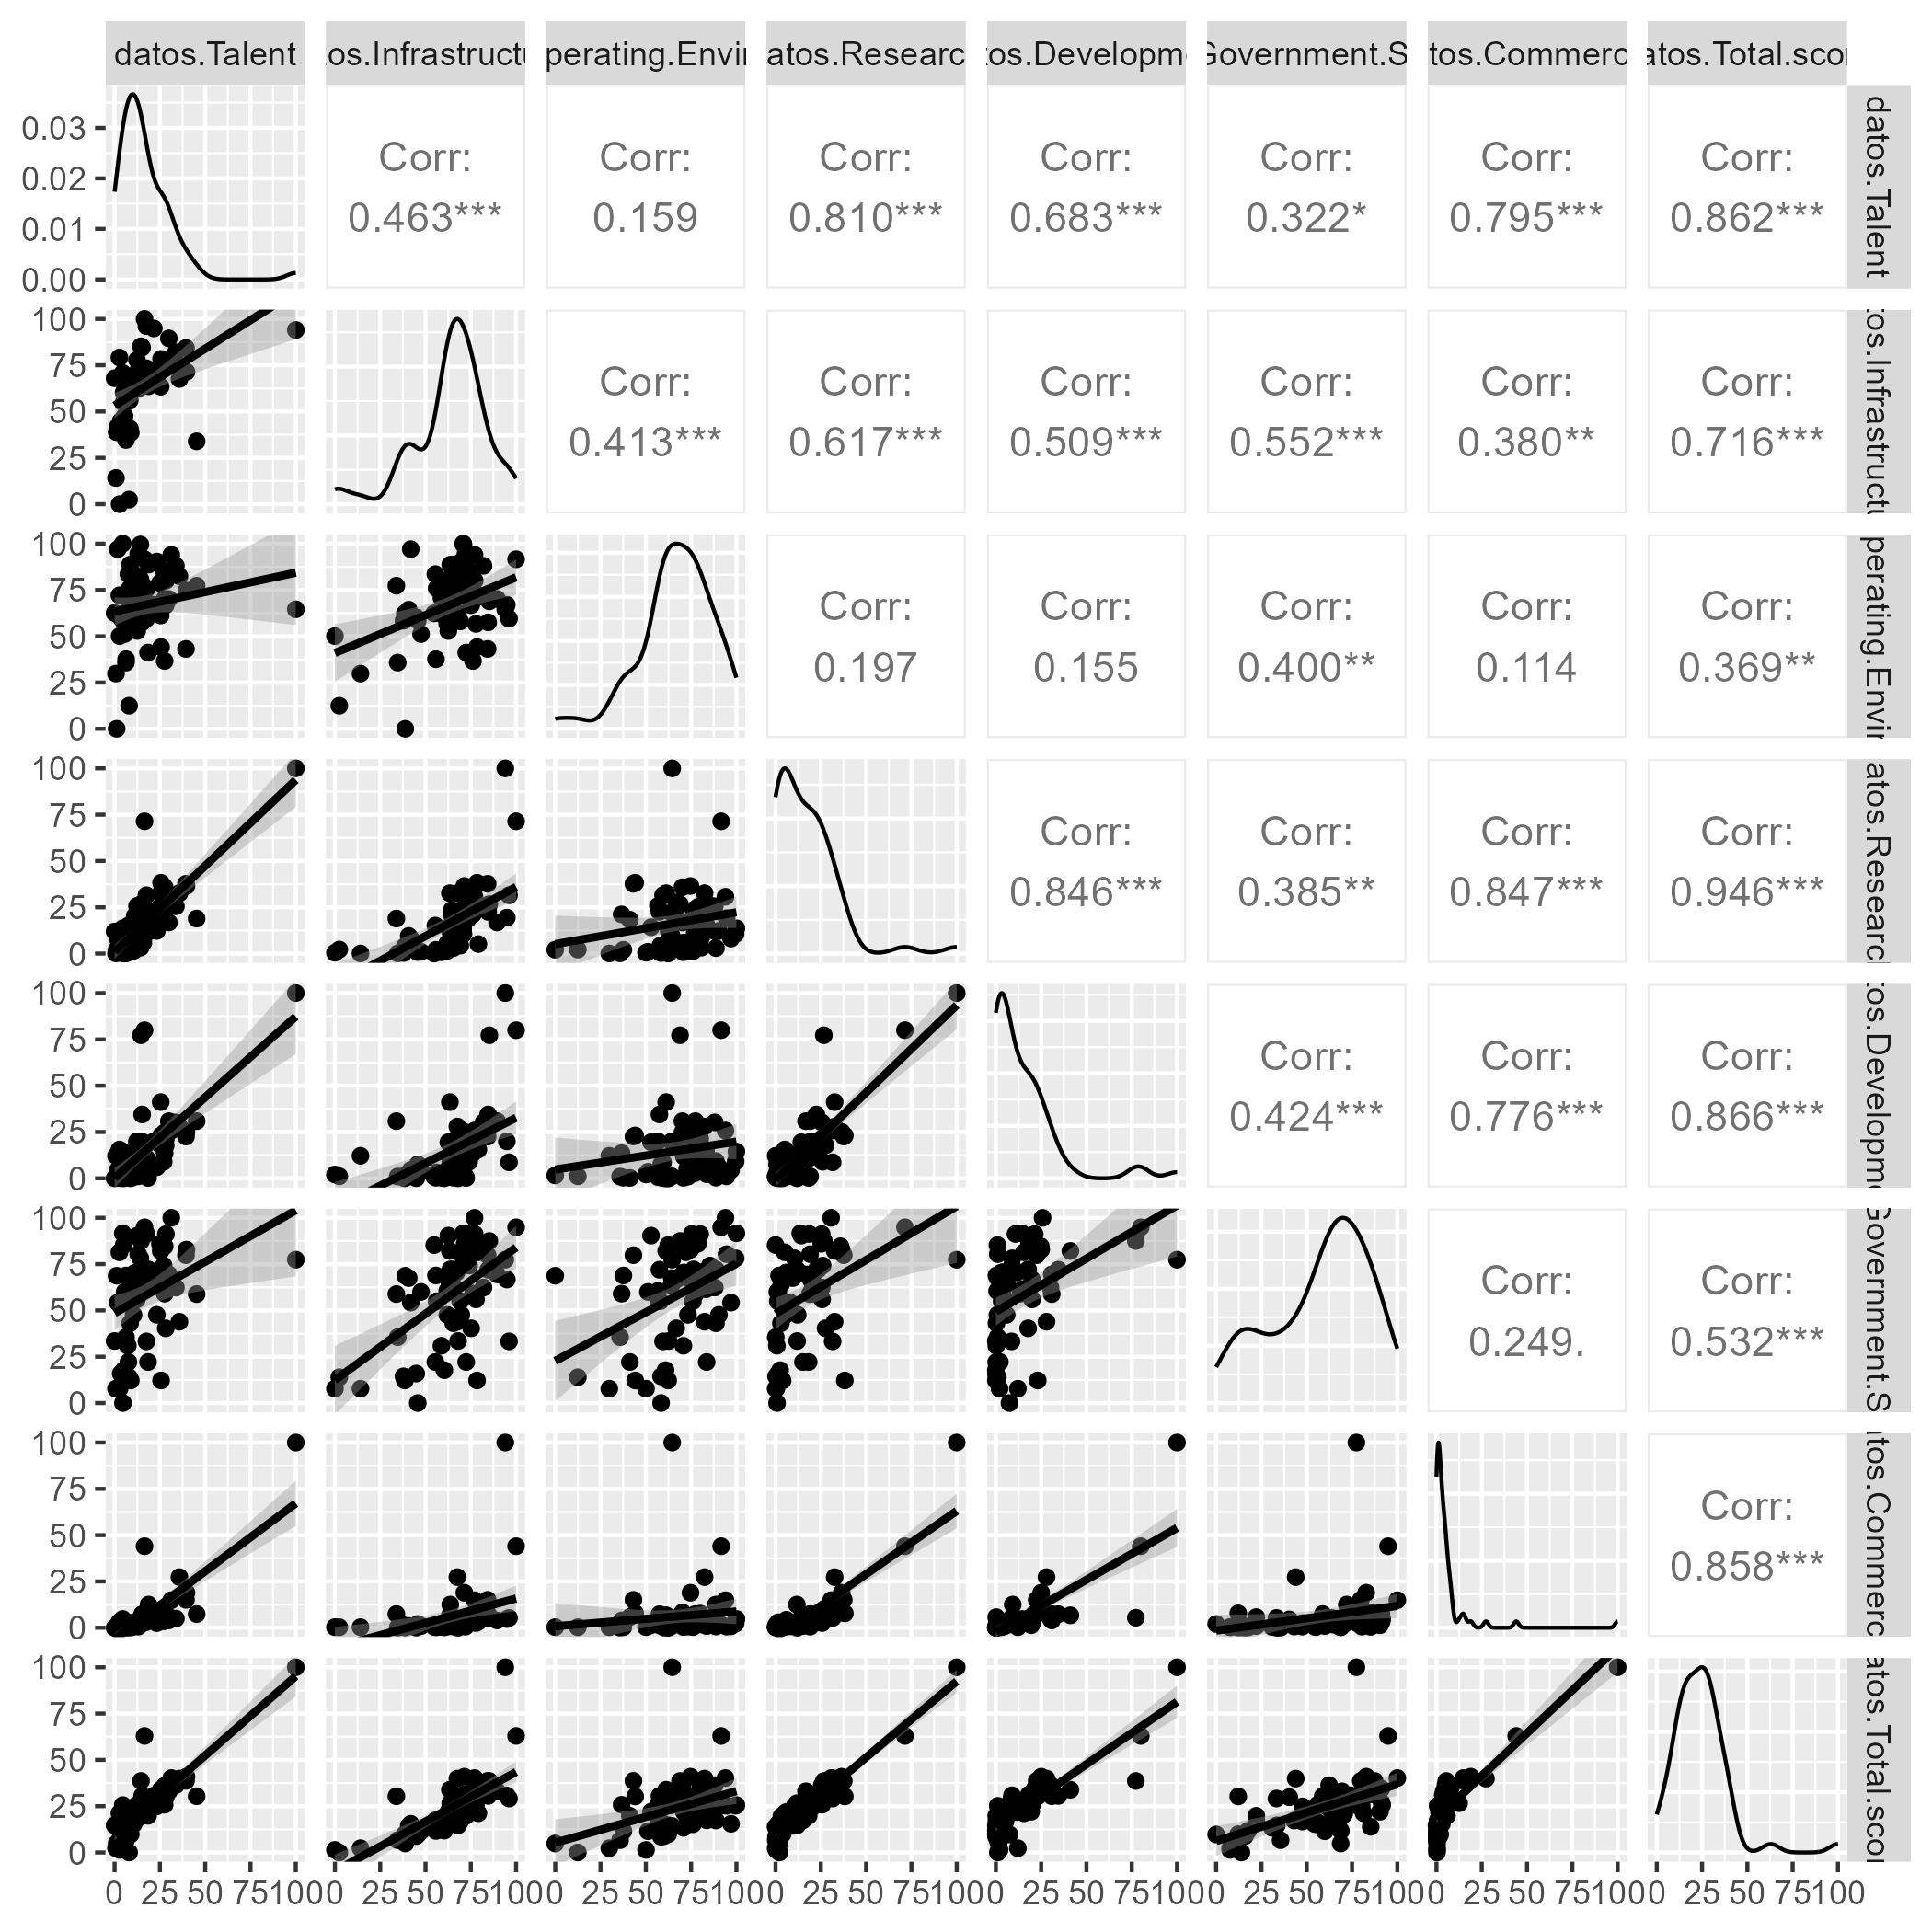
\includegraphics[width=\linewidth]{figura1.png}
\end{center}
Figura 1. Correlación lineal de Pearson índices.

\section*{Población y Muestra} % Using \section* for unnumbered sections
La población considerada para este estudio corresponde a los países y regiones incluidas en el AI Global Index.
La muestra se delimita a aquellos países con datos completos para las variables de interés:
inversión, infraestructura, talento, ambiente operativo e investigación y desarrollo.
Se seleccionaron X países según los criterios establecidos en la Figura 1, priorizando la disponibilidad
de datos confiables y actualizados.

\section*{Unidad de Análisis}
La unidad de análisis en este estudio es cada país individual, evaluado según las variables cuantitativas y cualitativas
definidas en la Tabla 1.

\section*{Criterios de Selección}
Los criterios considerados para la selección de los países y regiones incluyen:
\begin{enumerate}
    \item Disponibilidad de datos en el AI Global Index.
    \item Inclusión en las categorías de clasificación establecidas (ver Tabla 1).
    \item Representación geográfica equilibrada para evitar sesgos regionales.
\end{enumerate}

\section*{Tipo de Análisis}
El análisis realizado incluye:
\begin{itemize}
    \item Estadísticas descriptivas: medidas de tendencia central, dispersión y posición.
    \item Correlación lineal de Pearson entre las variables cuantitativas y el índice total.
    \item Comparación de medias para evaluar diferencias significativas entre subgrupos de países (por ejemplo, según ingresos).
\end{itemize}

Posteriormente, se emplearon métodos de análisis multivariado para explorar relaciones más complejas entre las variables,
como el análisis de componentes principales (ACP) para identificar patrones latentes en los datos.

\section{Resultados}
En la Tabla 2 se presentan las medidas de tendencia central y posición de las variables cuantitativas Índice Commerce, Research y Talent discriminadas de forma regional. 

Para casi todos los casos, la medida de tendencia central moda presentó más de tres valores, lo cuál no brinda mucha información acerca de los datos. En el caso de la media y mediana en Americas y Middle East, todos los índices difieren drásticamente, lo cuál indica que la distribución de los datos no es normal. En el caso Asia-Pacific, para el indicador Research y Total Score hay una alta cercanía entre estos indicadores, planteando la posibilidad de una distribución de campana, sin embargo esto debe ser confirmado gráficamente o mediante una prueba de simetría. Esto mismo ocurre para Europe con todos los indicadores, y en el caso del indicador Commerce hay una moda única que también es significativamente cercana a la media y mediana. Finalmente para Africa se presenta una alta cercanía de la mediana y la media en los índices Commerce, Talent y Research.

El mínimo en todas las regiones para todos los ídices es menor a 10, excepto Total Score de Americas con un 13.27, por otro lado, el máximo entre regiones presenta discrepancias más significativas, donde el el caso de Americas el máximo es 100 para todos los índices, en Asia-Pacific todos los máximos se encuentran por encima de 40, mientras en Europe los máximos de todos los índices se ubican en 40.93 o menos, al igual que Middle East. En el caso de Africa, toos los máximos de los indicadores se encuentran por debajo de 10.

\end{multicols}

\renewcommand{\arraystretch}{1.3}
\begin{scriptsize}
\begin{longtable}[t]{llrrrrrrr}
\caption{\label{tab:tabla2}Medidas de tendencia central y posición}\\
\toprule
Región & Índice & Media & Moda & Mínimo & Q1 & Mediana & Q3 & Máximo\\
\midrule
Americas & Commerce & 15.15 & > 3 modas & 0.34 & 0.48 & 1.07 & 5.93 & 100.00\\
Americas & Talent & 22.21 & > 3 modas & 1.72 & 6.70 & 9.48 & 17.91 & 100.00\\
Americas & Research & 18.39 & > 3 modas & 0.00 & 1.12 & 3.16 & 13.75 & 100.00\\
Americas & Total Score & 29.03 & > 3 modas & 13.27 & 14.89 & 15.41 & 24.22 & 100.00\\
Asia-Pacific & Commerce & 7.03 & > 3 modas & 0.09 & 0.70 & 3.92 & 7.16 & 44.02\\
\addlinespace
Asia-Pacific & Talent & 17.58 & > 3 modas & 5.51 & 8.61 & 14.86 & 21.87 & 45.27\\
Asia-Pacific & Research & 20.72 & > 3 modas & 0.12 & 3.02 & 20.72 & 30.30 & 71.42\\
Asia-Pacific & Total Score & 25.79 & > 3 modas & 0.00 & 12.88 & 27.45 & 33.03 & 62.92\\
Europe & Commerce & 4.28 & 3.08 & 0.61 & 1.75 & 3.46 & 4.97 & 18.91\\
Europe & Talent & 18.92 & > 3 modas & 6.69 & 12.46 & 16.97 & 27.07 & 39.65\\
\addlinespace
Europe & Research & 17.86 & > 3 modas & 0.28 & 10.60 & 18.60 & 25.21 & 38.24\\
Europe & Total Score & 25.49 & > 3 modas & 8.49 & 20.31 & 25.52 & 30.73 & 40.93\\
Middle East & Commerce & 5.97 & > 3 modas & 0.00 & 0.26 & 1.77 & 4.35 & 27.33\\
Middle East & Talent & 8.17 & > 3 modas & 0.00 & 1.50 & 3.57 & 4.86 & 35.76\\
Middle East & Research & 11.32 & > 3 modas & 2.08 & 3.18 & 8.54 & 13.21 & 32.63\\
\addlinespace
Middle East & Total Score & 19.66 & > 3 modas & 4.83 & 12.51 & 17.91 & 24.49 & 39.89\\
Africa & Commerce & 0.58 & > 3 modas & 0.10 & 0.15 & 0.31 & 0.33 & 2.03\\
Africa & Talent & 4.08 & > 3 modas & 0.75 & 2.74 & 3.36 & 4.61 & 8.94\\
Africa & Research & 1.34 & > 3 modas & 0.07 & 0.45 & 0.83 & 1.46 & 3.90\\
Africa & Total Score & 6.43 & > 3 modas & 1.38 & 2.30 & 8.87 & 9.71 & 9.87\\
\bottomrule
\end{longtable}

\end{scriptsize}\renewcommand{\arraystretch}{1}

\begin{multicols}{2}

En la Tabla 3 se presentan las medidas de disperción, covarianza y correlación lineal de Pearson con respecto al Total Score (AI Global Index) de las variables cuantitativas Índice Commerce, Research y Talent discriminadas de forma regional. 

Americas presentan los rangos más amplios de todas las regiones que van desde 86.73 en Total Score hasta 100 en Research, para la maroría los demás casos de las regiones Asia-Pacific, Europe y Middle East, los rangos de los diferentes índices varían alrededor de 20 y 40 indicando menor variablidad de los datos con excepciones de los índices Research y Total Score de Asia-Pacific con 71.30 y  62.92 respectivamente. En el caso de Africa se presentan los rangos más bajos donde todos estàn por debajo de 10, lo cuál sugiere que los datos en la región se distribuyen de manera altamente compacta.

Con respecto al coeeficiente de variación se puede afirmar que para la mayoría de los casos los datos son heterogéneos al presentar un coeficiente de variación mayor a 50, sin embargo, el índice Talent y Total Score en Europe presentan variación significativa ya que el coeficiente de variación se encuentra en el rango de 10 a 50.

En el caso de la covarianza, esta es positiva para todas las variables, lo cuál plantea la posibilidad de que estas tengan una relación lineal directa con el índice Total Score. Esto es confirmado con el coeficiente de correlación de Pearson, donde un valor superior a 0.8 indica hay una relación muy significativa, lo cuál es cierto para todos los indicadores en Americas y Middle East, Research en Asia-Pacific y Talent y Research en Europe. Por otro lado, una coeficiente entre 0.6 y 0.78 indica una relación significativa, la cuál está presente en Europe para el indicador Commerce y en Africa para Talent y Research.


\end{multicols}

\renewcommand{\arraystretch}{1.3}
\begin{scriptsize}
\begin{longtable}[t]{llrrrrrl}
\caption{\label{tab:tabla3}Medidas de dispersión e indicadores por región e índice}\\
\toprule
Región & Índice & Rango & RIQ & Desv.est & CV & Cov Total Score & Corr Total Score\\
\midrule
Americas & Commerce & 99.66 & 5.45 & 34.63 & 228.58 & 1025.58 & 0.99\\
Americas & Talent & 98.28 & 11.21 & 32.68 & 147.14 & 976.48 & 1.00\\
Americas & Research & 100.00 & 12.63 & 34.50 & 187.60 & 1033.01 & 1.00\\
Americas & Total Score & 86.73 & 9.33 & 30.01 & 103.38 & 900.62 & 1.00\\
Asia-Pacific & Commerce & 43.93 & 6.46 & 11.43 & 162.59 & 154.14 & 0.84\\
\addlinespace
Asia-Pacific & Talent & 39.76 & 13.26 & 12.16 & 69.17 & 95.12 & 0.49\\
Asia-Pacific & Research & 71.30 & 27.28 & 19.60 & 94.59 & 298.15 & 0.95\\
Asia-Pacific & Total Score & 62.92 & 20.15 & 16.05 & 62.23 & 257.75 & 1.00\\
Europe & Commerce & 18.30 & 3.22 & 3.92 & 91.59 & 19.30 & 0.67\\
Europe & Talent & 32.96 & 14.61 & 8.71 & 46.04 & 57.84 & 0.91\\
\addlinespace
Europe & Research & 37.96 & 14.61 & 10.12 & 56.66 & 61.59 & 0.83\\
Europe & Total Score & 32.44 & 10.42 & 7.33 & 28.76 & 53.68 & 1.00\\
Middle East & Commerce & 27.33 & 4.09 & 10.64 & 178.22 & 115.90 & 0.89\\
Middle East & Talent & 35.76 & 3.37 & 13.65 & 167.07 & 139.71 & 0.83\\
Middle East & Research & 30.55 & 10.03 & 11.50 & 101.59 & 127.72 & 0.90\\
\addlinespace
Middle East & Total Score & 35.06 & 11.98 & 12.28 & 62.46 & 150.74 & 1.00\\
Africa & Commerce & 1.93 & 0.18 & 0.81 & 139.66 & 1.12 & 0.33\\
Africa & Talent & 8.19 & 1.87 & 3.05 & 74.75 & 9.30 & 0.72\\
Africa & Research & 3.83 & 1.01 & 1.52 & 113.43 & 4.29 & 0.67\\
Africa & Total Score & 8.49 & 7.41 & 4.22 & 65.63 & 17.78 & 1.00\\
\bottomrule
\end{longtable}

\end{scriptsize}\renewcommand{\arraystretch}{1}

\begin{multicols}{2}

\subsection{Índice Commerce}

En la Tabla 4 se presentan las frecuencias bivariadas del indice Commerce y el índice Total Score. En esta se puede apreciar como hay una alta concentración de los datos en la parte superior izquierda de la tabla, donde se indica que 55 de los 62 datos con un Índice Commerce entre 0 y 10 presentan un Total Score menor o igual a 40.

60 de los 62 datos de los diferentes países presentan un Índice Commerce menor o igual a 30, indicando que la inversión e iniciativas comerciales de Inteligencia Artificial en el 96\% de los países estudiados es baja.

Hay un dato con un Índice Commerce entre 40 y 50 con un total score correspondiente en el rango de 60 y 70. El último dato presenta un Índice Commerce entre 90 y 100 y un Total Score entre 90 y 100, planteando claramente la presencia de un dato atípico por su gran lejanía de los demás datos obtenidos de los países estudiados.

\end{multicols}

\renewcommand{\arraystretch}{1.3}
\begin{scriptsize}% latex table generated in R 4.4.2 by xtable 1.8-4 package
<<<<<<< HEAD
% Wed Apr 16 20:46:01 2025
=======
% Wed Apr 16 20:42:52 2025
>>>>>>> 491d84188ebb9437248195356dc298d3a269b661
\begin{longtable}{lrrrrrrrrrrr}
\caption{Tabla de Frecuencia Bivariada Índice Commerce (A) vs Total Score (B)} \\ 
  \hline
A   -   B & [0, 10] & (10, 20] & (20, 30] & (30, 40] & (40, 50] & (50, 60] & (60, 70] & (70, 80] & (80, 90] & (90, 100] & Total \\ 
  \hline
(0, 10] & 9.00 & 17.00 & 17.00 & 12.00 & 0.00 & 0.00 & 0.00 & 0.00 & 0.00 & 0.00 & 55.00 \\ 
  (10, 20] & 0.00 & 0.00 & 1.00 & 1.00 & 2.00 & 0.00 & 0.00 & 0.00 & 0.00 & 0.00 & 4.00 \\ 
  (20, 30] & 0.00 & 0.00 & 0.00 & 1.00 & 0.00 & 0.00 & 0.00 & 0.00 & 0.00 & 0.00 & 1.00 \\ 
  (30, 40] & 0.00 & 0.00 & 0.00 & 0.00 & 0.00 & 0.00 & 0.00 & 0.00 & 0.00 & 0.00 & 0.00 \\ 
  (40, 50] & 0.00 & 0.00 & 0.00 & 0.00 & 0.00 & 0.00 & 1.00 & 0.00 & 0.00 & 0.00 & 1.00 \\ 
  (50, 60] & 0.00 & 0.00 & 0.00 & 0.00 & 0.00 & 0.00 & 0.00 & 0.00 & 0.00 & 0.00 & 0.00 \\ 
  (60, 70] & 0.00 & 0.00 & 0.00 & 0.00 & 0.00 & 0.00 & 0.00 & 0.00 & 0.00 & 0.00 & 0.00 \\ 
  (70, 80] & 0.00 & 0.00 & 0.00 & 0.00 & 0.00 & 0.00 & 0.00 & 0.00 & 0.00 & 0.00 & 0.00 \\ 
  (80, 90] & 0.00 & 0.00 & 0.00 & 0.00 & 0.00 & 0.00 & 0.00 & 0.00 & 0.00 & 0.00 & 0.00 \\ 
  (90, 100] & 0.00 & 0.00 & 0.00 & 0.00 & 0.00 & 0.00 & 0.00 & 0.00 & 0.00 & 1.00 & 1.00 \\ 
  Total & 9.00 & 17.00 & 18.00 & 14.00 & 2.00 & 0.00 & 1.00 & 0.00 & 0.00 & 1.00 & 62.00 \\ 
   \hline
\hline
\end{longtable}
\end{scriptsize}\renewcommand{\arraystretch}{1}

\begin{multicols}{2}

El histograma presentado en la Figura 2 permite plasmar gráficamente la distribución de los datos de la variable índince Commerce. Su puede observar como en los casos de Americas, Asia-Pacific y Middle East los datos se encuentran concentrados hacia la izquierda del eje x, sin embargo presentan una asimetría positiva o sesgo a la derecha, donde la media es mayor a la mediana, indicando que posiblemente se presenten puntos atípicos hacia la derecha del eje x.

En el caso de Europe, se observa que los datos se agrupan hacia la izquierda del eje x, sin embargo, aunque en el análisis de la Tabla 2 se teorizaba una posible distribución normal debido a la cercanía de la media, mediana y moda, no se muestra simetría en la gráfica y se presenta una distribución con mayor similitud a una exponencial.

En el caso de Africa, los datos se encuentran concentrados alrededor del 0, mostrando una distribución altamente compacta sin embargo el gráfico no permite confirmar la forma de distribión de los datos. 




\begin{center}
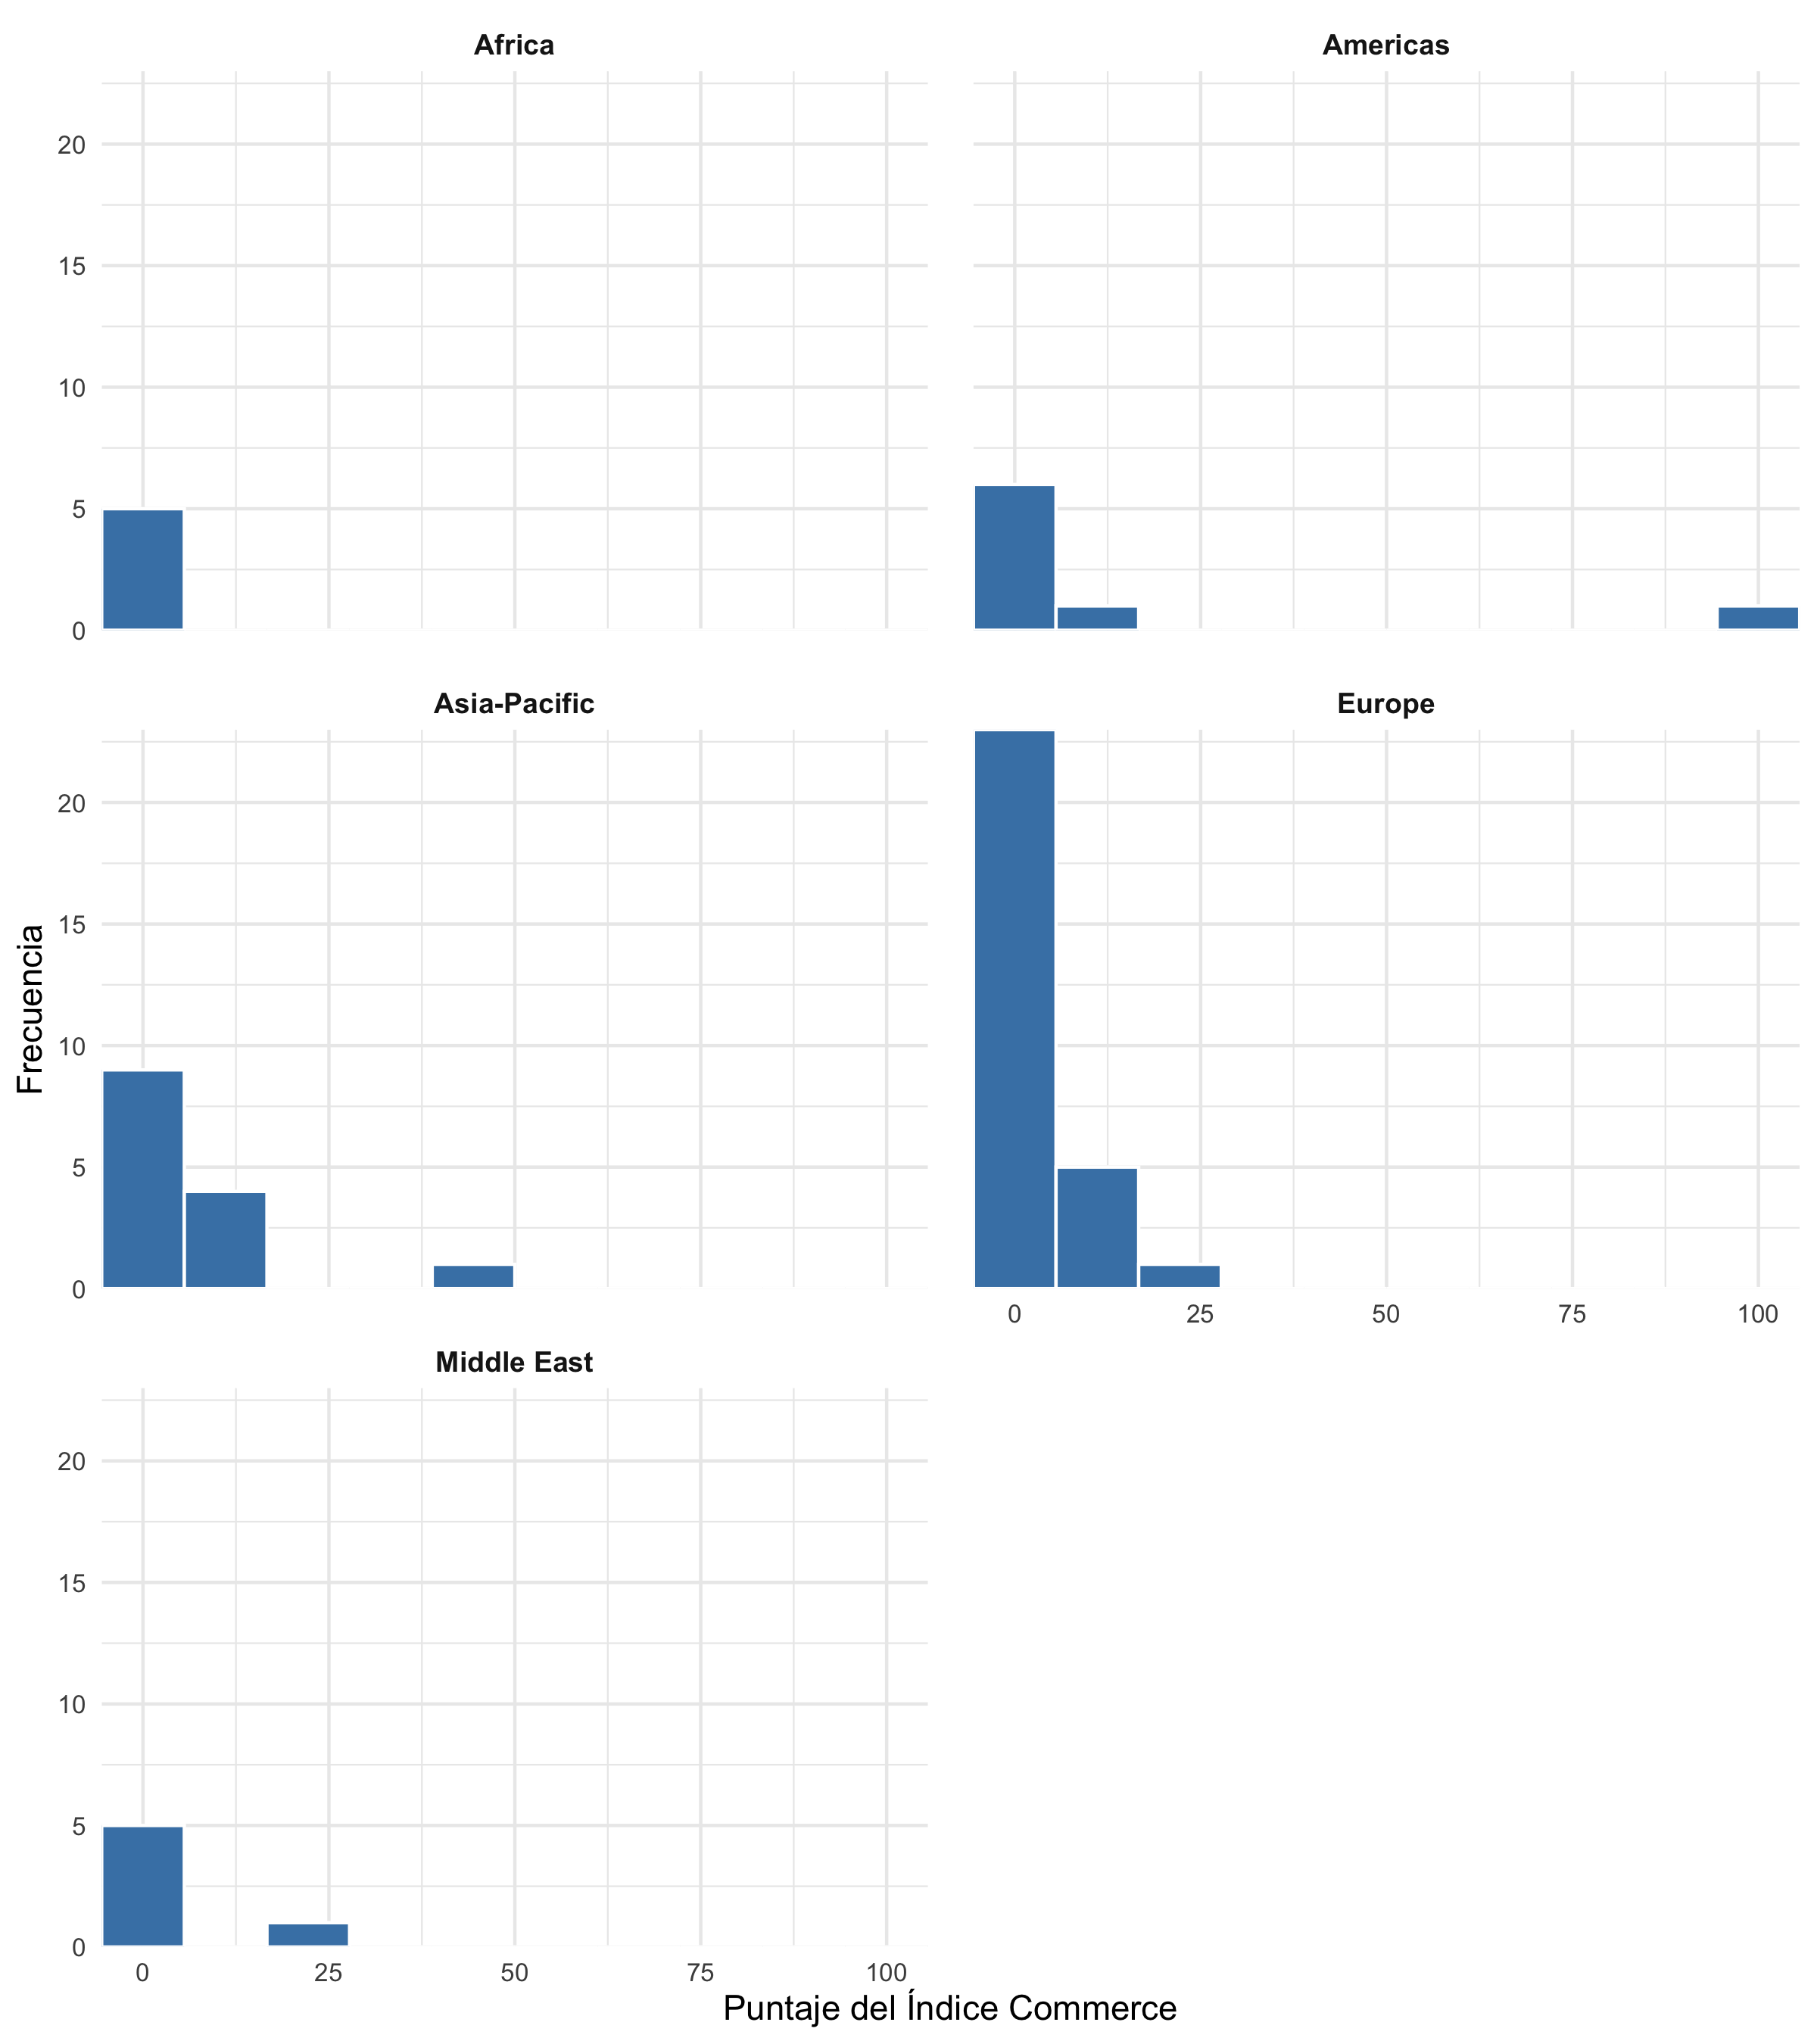
\includegraphics[width=\linewidth]{figura2.png}
\end{center}
Figura 2. Distribución del Índice Commerce agrupado por Región.


La Ojiva en la Figura 3 presenta la distriución acumulada de los datos de manera porcental, lo cuál permite estimar los percentiles correspondientes a los diferentes puntajes del índice Commerce.

En el caso de Americas, al rededor del 87.5\% de los datos tienen un índice Commmerce alrededor de 13 o menos, lo cuál indica una alta concentración de los datos a la izquierda del eje, sin embargo se presenta un salto abrupto en el índice que se distancia de los demás datos, indicando un posible dato atípico en el puntaje 100. Esto mismo ocurre en Middle East donde aproximadamente un 80\% de los datos tienen un puntaje de alrededor de 7 o menos y se presenta salto abrupto en el índice a un puntaje alrededor de 27.

Asia-Pacific y Europe presentan distribuciones similares, sin embargo en Europe los datos se ven más concentrados a la izquierda del eje. En ambos casos una mayoría cercana a 85\% de los datos tienen un índice de aproximadmente 20 o menos en Asia-Pacific y 10 o menos en Europe. Posteriormente a este punto se presenta un incremento gradual en los puntajes para los datos restantes.

En África cerca del 80\% de los datos están concentrados en un puntaje cercano a 0, lo cuál indica que posiblemente no hay simetría en la distribución por lo cuál esta no es normal.




\begin{center}
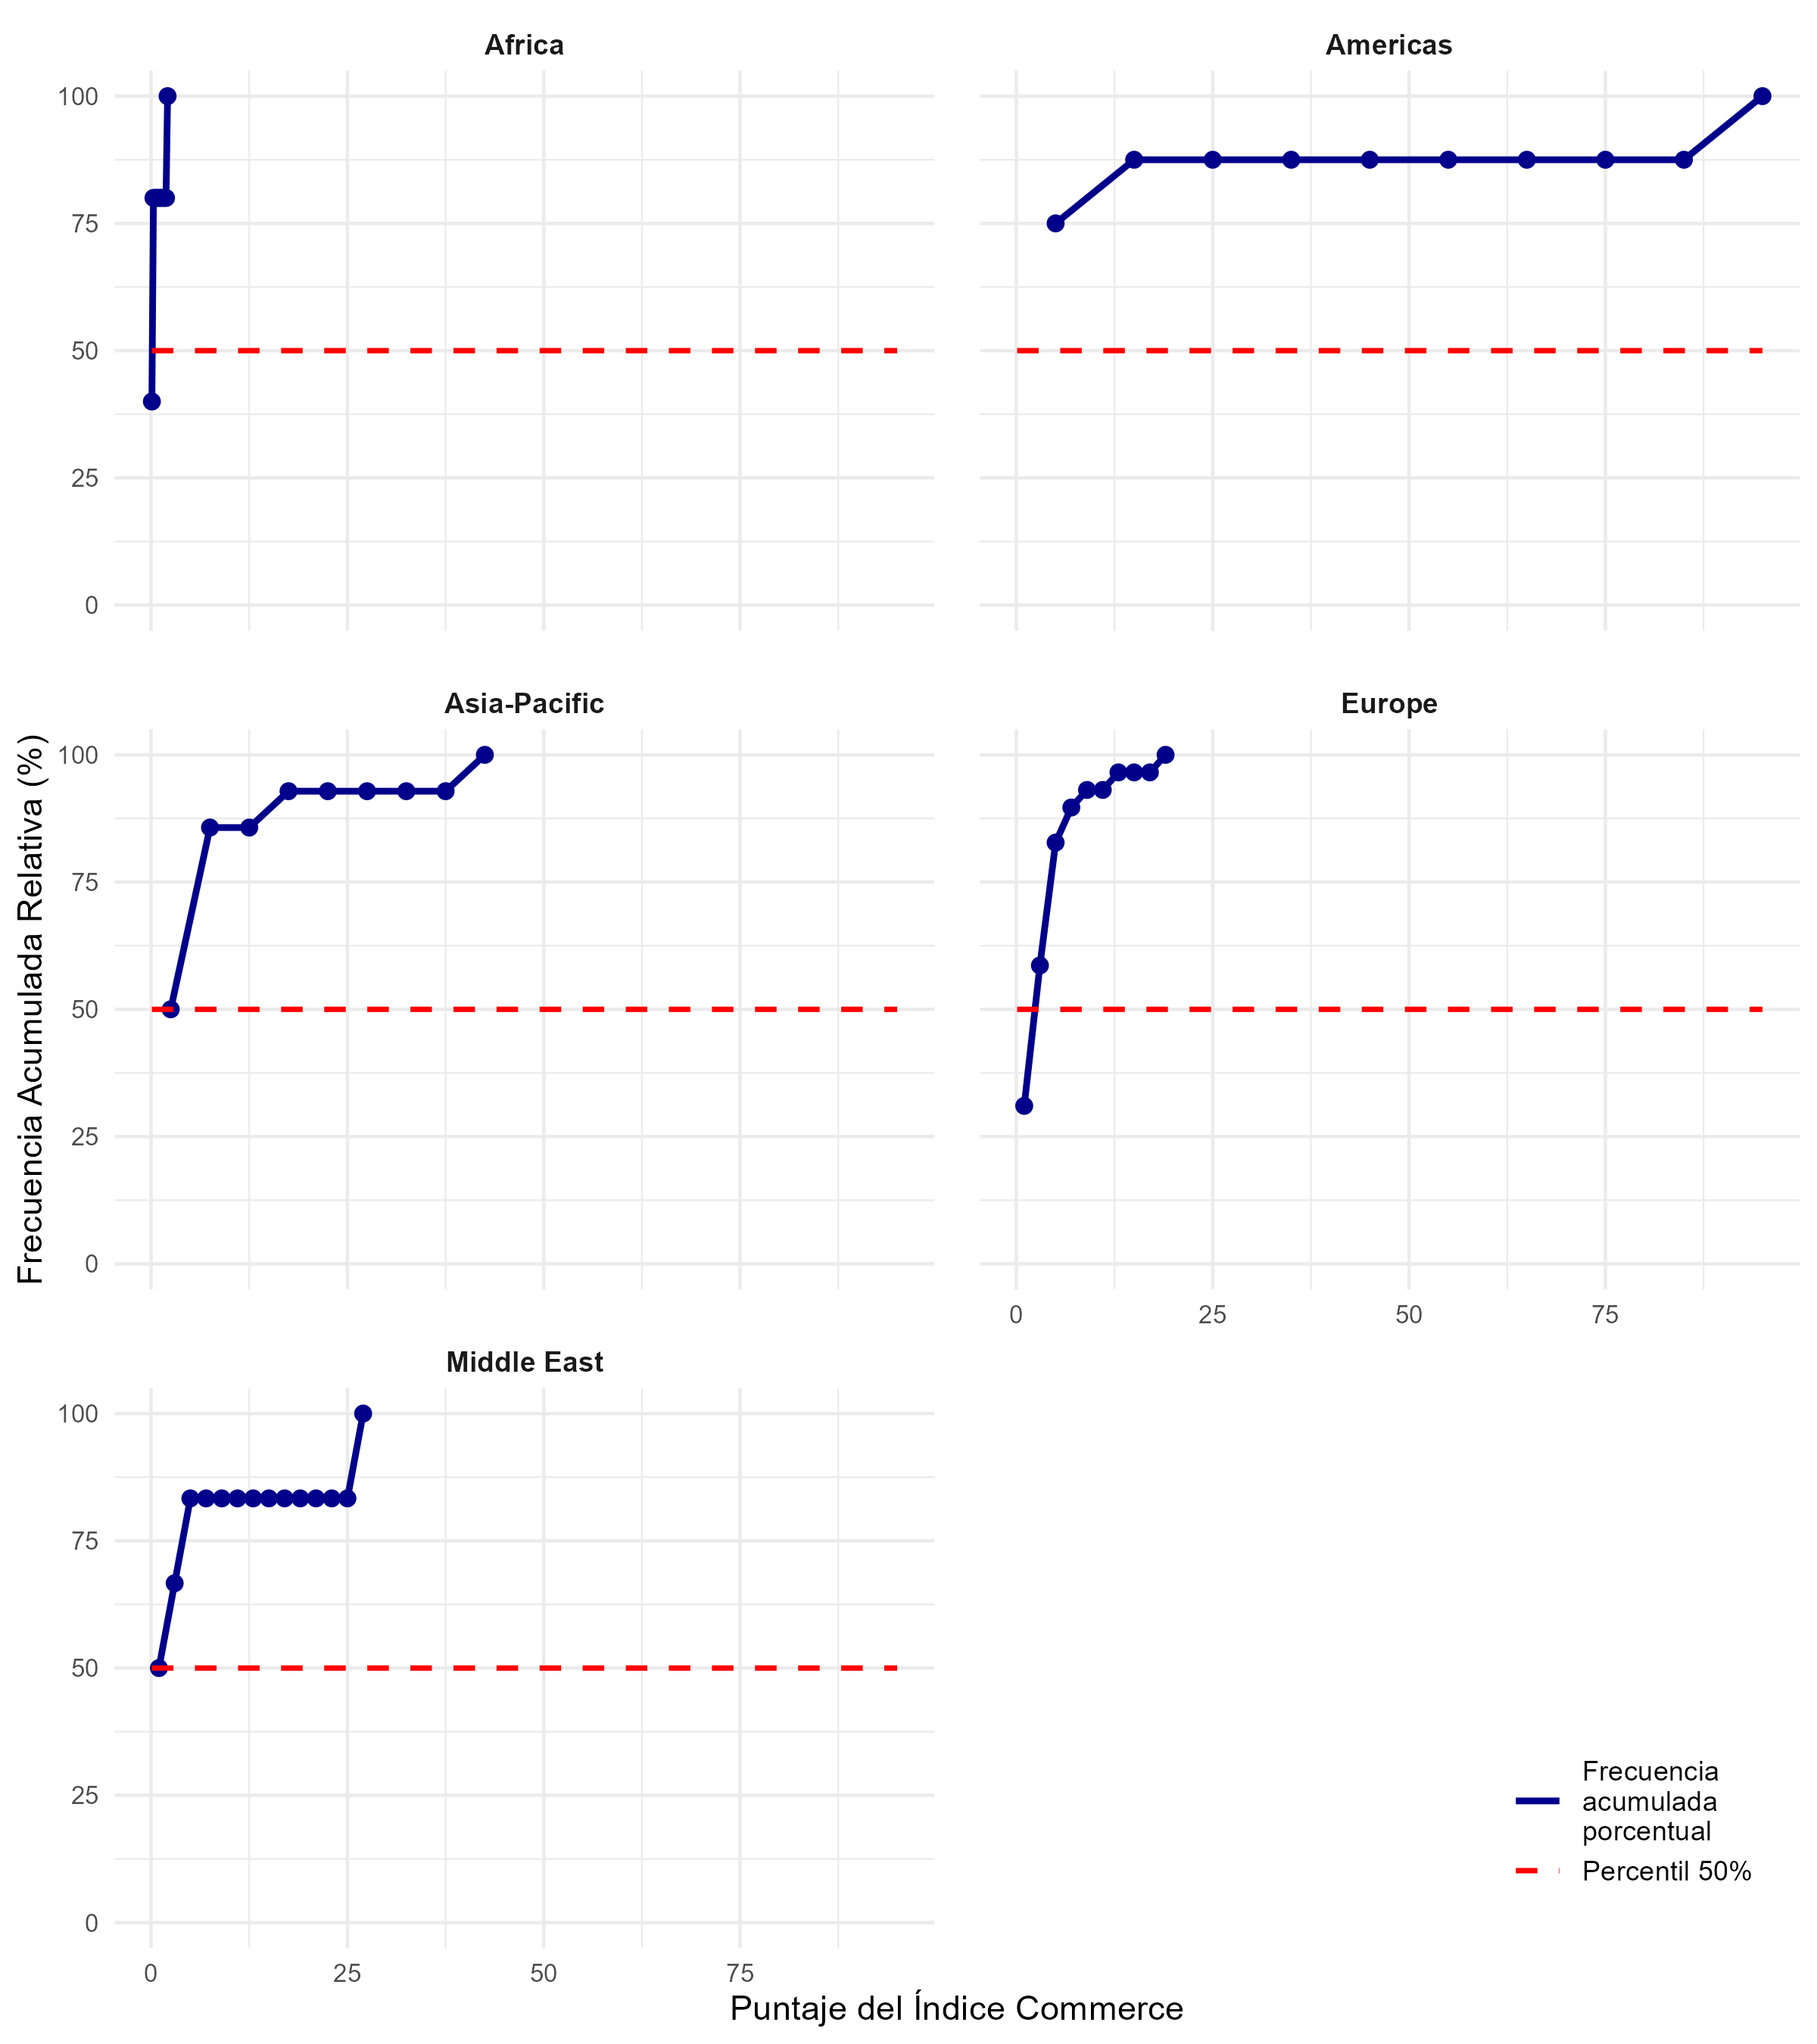
\includegraphics[width=\linewidth]{figura3.png}
\end{center}
Figura 3. Distribución acumulada del Índice Commerce agrupado por Región.


El diagrama de cajas y bigotes presentado en la Figura 4 presenta gráficamente las medidas de posición del Índice Commerce, la media e identifica los datos atípicos.

En el caso de Africa se muestra una muy alta compacidad de los datos donde la media es cercana a la mediana, cuartiles 1 y 3 y los límites inferiores y superiores de los bigotes. En este caso se presenta un dato atípico que se encuentra en relativa cercanía del límite superior del bigote.

En el caso de Americas se observa como el 50\% de los datos son altamente compactos, los datos entre la mediana y el Q3 tienen una disperción más alta y la media se aleja en gran medida (con un valor más alto que el límite superior del bigote) de la mediana debido a la presencia de 1 dato atípico a una gran distancia del resto de los datos al presentar un índice de 100. Esto también se observa en Asia-Pacific y Middle East, sin embargo en estos casos aunque hay un dato atípico que aleja la media del resto de los datos, la media se encuentra en un valor cercano al cuartil tres.

En el caso de Europe los datos se distribuyen de manera significativamente compacta. Aunque se presentan dos datos atípicos, la media se mantiene en relativa cercanía con la mediana.




\begin{center}
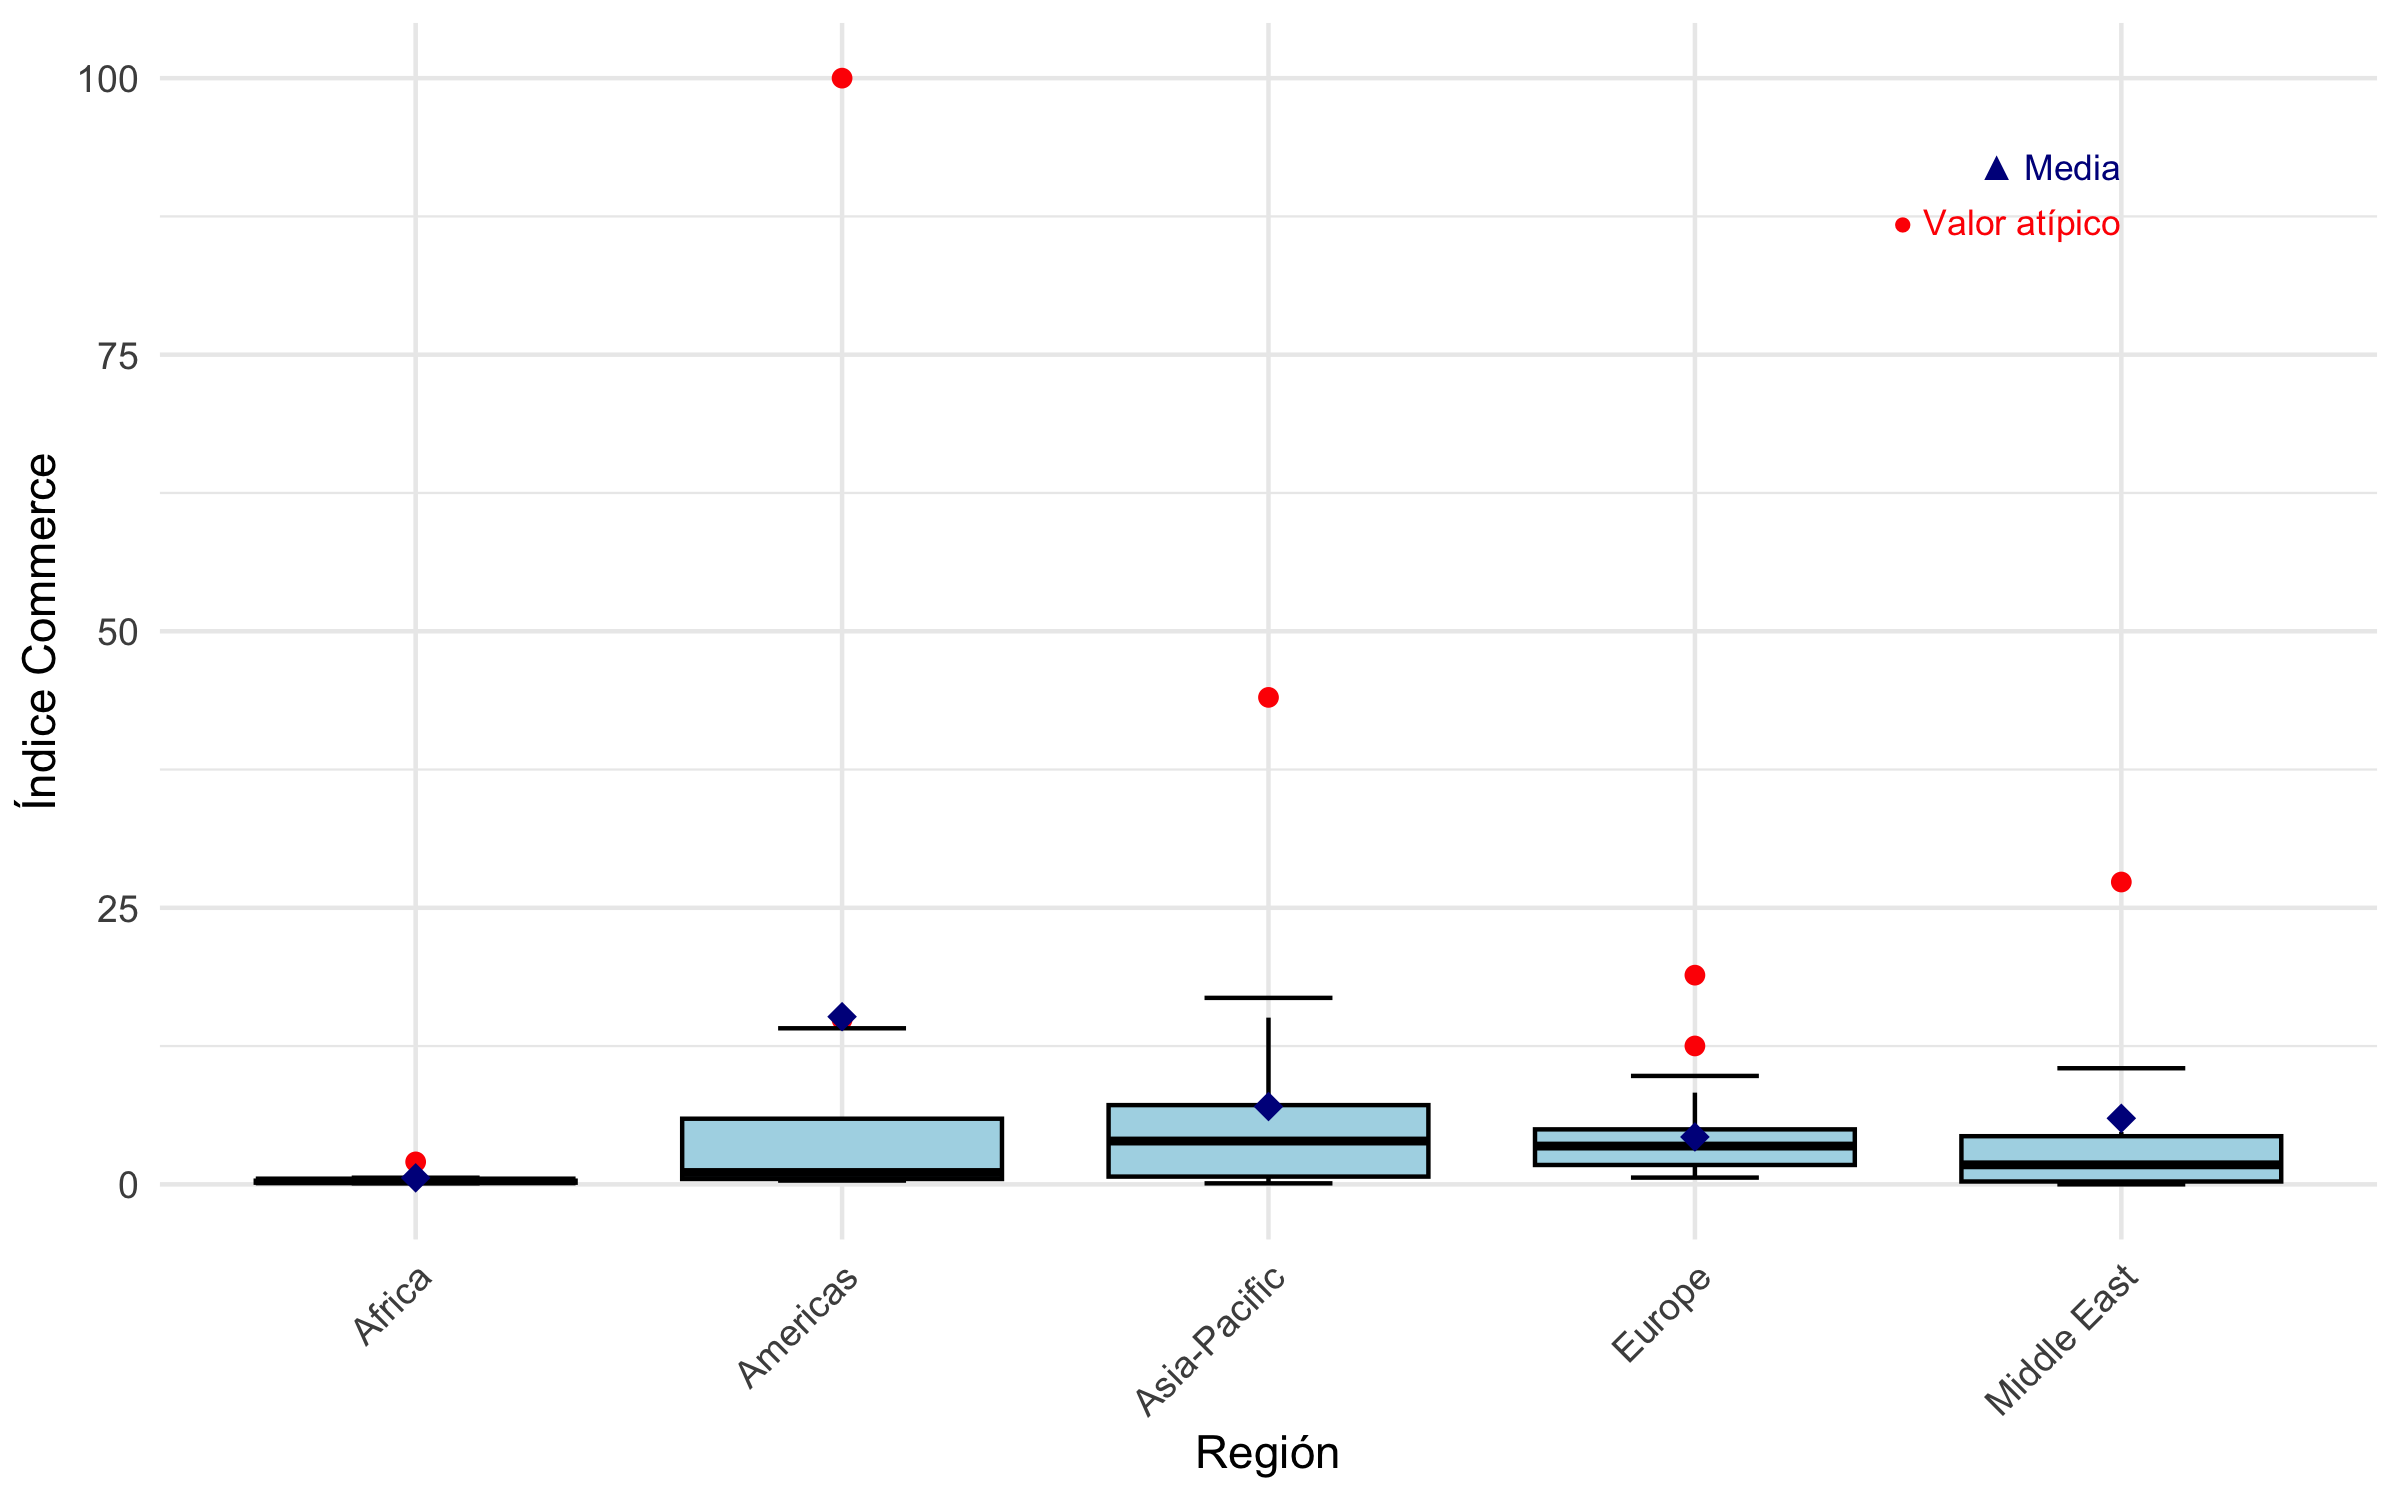
\includegraphics[width=\linewidth]{figura4.png}
\end{center}

El indicador Commercial evalúa la capacidad de los países para convertir el conocimiento en IA en aplicaciones comerciales y soluciones de mercado. La Tabla 5 presenta la distribución global de este indicador a través de intervalos de 10 puntos, mostrando las frecuencias absolutas y relativas de países en cada rango. Este análisis es clave para identificar qué economías están liderando la comercialización de tecnologías de IA y qué regiones necesitan fortalecer sus ecosistemas de innovación empresarial.

\end{multicols}

\begin{longtable}[]{@{}lcccc@{}}
\caption{Frecuencia del Índice Commercial}\tabularnewline
\toprule\noalign{}
Intervalo & F.Absoluta & F.Relativa & F.Abs.Acum & F.Rel.Acum \\
\midrule\noalign{}
\endfirsthead
\toprule\noalign{}
Intervalo & F.Absoluta & F.Relativa & F.Abs.Acum & F.Rel.Acum \\
\midrule\noalign{}
\endhead
\bottomrule\noalign{}
\endlastfoot
{[}0,10{]} & 55 & 0.89 & 55 & 0.89 \\
(10,20{]} & 4 & 0.06 & 59 & 0.95 \\
(20,30{]} & 1 & 0.02 & 60 & 0.97 \\
(30,40{]} & 0 & 0.00 & 60 & 0.97 \\
(40,50{]} & 1 & 0.02 & 61 & 0.98 \\
(50,60{]} & 0 & 0.00 & 61 & 0.98 \\
(60,70{]} & 0 & 0.00 & 61 & 0.98 \\
(70,80{]} & 0 & 0.00 & 61 & 0.98 \\
(80,90{]} & 0 & 0.00 & 61 & 0.98 \\
(90,100{]} & 1 & 0.02 & 62 & 1.00 \\
\end{longtable}

\begin{multicols}{2}

\subsection{Índice Research}

El indicador *Research* mide la producción científica y capacidad investigadora en inteligencia artificial, siendo un predictor clave del desarrollo tecnológico futuro. La Tabla 5 presenta su distribución global mediante frecuencias absolutas y relativas, permitiendo identificar los patrones de concentración del conocimiento especializado. Este análisis es fundamental para comprender qué países están liderando la generación de nuevo conocimiento en IA y qué regiones requieren fortalecer sus sistemas de investigación.

La Tabla 6 revela una concentración extrema en la capacidad comercial, con más del 65\% de los países ubicados por debajo de los 20 puntos (F.Rel.A = 0.65). Solo un pequeño grupo de naciones, liderado por Estados Unidos (100 puntos), supera los 80 puntos, demostrando su dominio en la transformación de investigación en productos comerciales. Los resultados destacan la brecha entre los polos tecnológicos consolidados y el resto del mundo, particularmente en regiones como África y Latinoamérica.

\end{multicols}

\begin{longtable}[]{@{}lcccc@{}}
\caption{Frecuencia del Índice Research}\tabularnewline
\toprule\noalign{}
Intervalo & F.Absoluta & F.Relativa & F.Abs.Acum & F.Rel.Acum \\
\midrule\noalign{}
\endfirsthead
\toprule\noalign{}
Intervalo & F.Absoluta & F.Relativa & F.Abs.Acum & F.Rel.Acum \\
\midrule\noalign{}
\endhead
\bottomrule\noalign{}
\endlastfoot
{[}0,10{]} & 26 & 0.42 & 26 & 0.42 \\
(10,20{]} & 14 & 0.23 & 40 & 0.65 \\
(20,30{]} & 12 & 0.19 & 52 & 0.84 \\
(30,40{]} & 8 & 0.13 & 60 & 0.97 \\
(40,50{]} & 0 & 0.00 & 60 & 0.97 \\
(50,60{]} & 0 & 0.00 & 60 & 0.97 \\
(60,70{]} & 0 & 0.00 & 60 & 0.97 \\
(70,80{]} & 1 & 0.02 & 61 & 0.98 \\
(80,90{]} & 0 & 0.00 & 61 & 0.98 \\
(90,100{]} & 1 & 0.02 & 62 & 1.00 \\
\end{longtable}

\begin{multicols}{2}

Los resultados revelan una concentración extrema en la capacidad investigadora: mientras el 60\% de los países se ubica por debajo de los 30 puntos (F.Rel.Acum = 0.60), solo un selecto grupo (15\%) supera los 70 puntos. Estados Unidos (100 puntos) y China (71.42) dominan claramente los intervalos superiores. Sin embargo, destaca que varios países europeos (Reino Unido 36.5, Alemania 35.84) mantienen capacidades significativas. La presencia casi nula de países africanos y latinoamericanos por encima de los 20 puntos (F.Abs = 2) evidencia un riesgo crítico de dependencia tecnológica.

\subsection{Índice Talent}
tabla de frecuencia bivariada (indice vs total socore)
histograma x region
ojiva x region
diagrama de cajas y bigotes x region

La Tabla 7 revela una distribución desigual del talento en IA a nivel mundial, con una marcada concentración en los extremos: mientras el 42\% de los países se ubica en el rango más bajo (0-20 puntos), solo un 18 pot ciento supera los 50 puntos. Las frecuencias acumuladas muestran que apenas el 30 por ciento de las naciones alcanza niveles competitivos (mayor igual a 40 puntos), destacando Estados Unidos (100 puntos) como caso excepcional. Esta polarización refleja brechas estructurales en la formación de profesionales calificados, donde economías desarrolladas capturan la mayor parte del talento global.

\end{multicols}

\begin{longtable}[]{@{}lcccc@{}}
\caption{Frecuencia del Índice Talent}\tabularnewline
\toprule\noalign{}
Intervalo & F.Absoluta & F.Relativa & F.Abs.Acum & F.Rel.Acum \\
\midrule\noalign{}
\endfirsthead
\toprule\noalign{}
Intervalo & F.Absoluta & F.Relativa & F.Abs.Acum & F.Rel.Acum \\
\midrule\noalign{}
\endhead
\bottomrule\noalign{}
\endlastfoot
{[}0,10{]} & 22 & 0.35 & 22 & 0.35 \\
(10,20{]} & 22 & 0.35 & 44 & 0.71 \\
(20,30{]} & 11 & 0.18 & 55 & 0.89 \\
(30,40{]} & 5 & 0.08 & 60 & 0.97 \\
(40,50{]} & 1 & 0.02 & 61 & 0.98 \\
(50,60{]} & 0 & 0.00 & 61 & 0.98 \\
(60,70{]} & 0 & 0.00 & 61 & 0.98 \\
(70,80{]} & 0 & 0.00 & 61 & 0.98 \\
(80,90{]} & 0 & 0.00 & 61 & 0.98 \\
(90,100{]} & 1 & 0.02 & 62 & 1.00 \\
\end{longtable}

\begin{multicols}{2}

La Tabla 6 revela una fuerte desigualdad en la distribución global de talento en IA. Estados Unidos destaca como líder absoluto (100 puntos), mientras que más del 40 por ciento de los países se concentra en el nivel más bajo (0-20 puntos). Esta brecha refleja las profundas asimetrías en desarrollo tecnológico, donde solo un puñado de naciones concentra las capacidades avanzadas.

La escasez de países en rangos intermedios (30-60 puntos) es particularmente preocupante, pues muestra que pocas economías están logrando desarrollar talento competitivo. Estos resultados subrayan la urgencia de políticas globales para democratizar el acceso a formación especializada, especialmente en regiones en desarrollo donde el talento en IA resulta crítico para no quedar rezagados en la transformación digital.

\subsection{Región}


El diagrama de torta de distribución regional proporciona el contexto geopolítico esencial para interpretar las desigualdades en los indicadores de IA (Talent-Research-Commercial), revelando que la excelencia tecnológica no se distribuye aleatoriamente, sino que se concentra en regiones con ventajas históricas de inversión en educación e innovación. Esta visualización evidencia cómo la mayor representación proporcional de ciertas zonas (como América del Norte y Asia-Pacífico) correlaciona directamente con su dominio en los intervalos superiores de los tres indicadores, mientras que regiones con menor representación proporcional (África, Latinoamérica) aparecen sistemáticamente en los rangos inferiores, configurando un mapa de dependencia tecnológica global

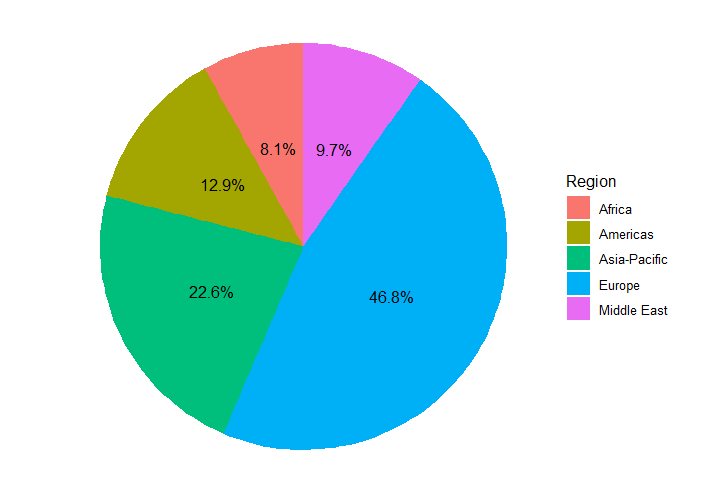
\includegraphics[width=\linewidth]{Efrain(torta).png}
Figura 4. Distribución porcentual por Región.

\section{Análisis de resultados}
El estudio realizado mediante tablas univariadas de frecuencias (absolutas, relativas y acumuladas) de los tres indicadores clave revela patrones estructurales preocupantes en el desarrollo global de la inteligencia artificial. El análisis muestra una concentración extrema de capacidades en un reducido grupo de países - principalmente Estados Unidos (con puntuaciones perfectas en Talent y Commercial), China (destacada en Research con 71.42 puntos) y algunas economías europeas -, que dominan simultáneamente los tres ámbitos. Esta triple brecha (formativa, científica y comercial), evidenciada por las frecuencias acumuladas donde el 80 por ciento de los países analizados muestra desempeños limitados (F.Rel.Acum mayor a 0.80 en intervalos menores a 30 puntos para los tres indicadores), crea un escenario crítico de dependencia tecnológica.

El estudio revela que solo el 12\% de los países (7/58) alcanza puntuaciones altas (mayores a 70 puntos) en los tres indicadores simultáneamente, mientras que el 65\% muestra limitaciones críticas en el Índice Commerce (F.Rel.Acum=0.65 en menos de 20 puntos), porcentaje que supera en 20 puntos al de Research (45\%). Destaca especialmente la brecha en Talent, donde Estados Unidos (100 puntos) quintuplica la media global (19.3 puntos), evidenciando una concentración extrema de capital humano especializado.

\section{Conclusiones}

\section{Referencias}
[1]   “AI Global Index,” Kaggle, Apr. 26, 2023.         https://www.kaggle.com/datasets/katerynameleshenko/ai-index

[2]   W. Navidi, Statistics for Engineers and Scientists w/ CD-ROM. McGraw-Hill Sci./Eng./Math, 2004.

\end{multicols}

\end{document}
